\documentclass[tikz,border=10pt]{standalone}
\usepackage{amsmath}
\usepackage{tikz}
\usetikzlibrary{arrows.meta,calc,positioning}

\tikzset{
  signal/.style={->, line width=1.2pt, draw=black!80, >=Stealth},
  block/.style={draw=blue!70!black, line width=1.2pt, rectangle, rounded corners=2pt, minimum width=2.2cm, minimum height=1.0cm, align=center, fill=none},
  sum/.style={draw=green!55!black, line width=1.2pt, circle, minimum size=0.6cm, inner sep=0pt, fill=none,
    path picture={
      \draw[green!55!black, line width=0.9pt]
      (path picture bounding box.south west) -- (path picture bounding box.north east)
      (path picture bounding box.north west) -- (path picture bounding box.south east);
    }},
  note/.style={font=\small, align=center}
}

\begin{document}
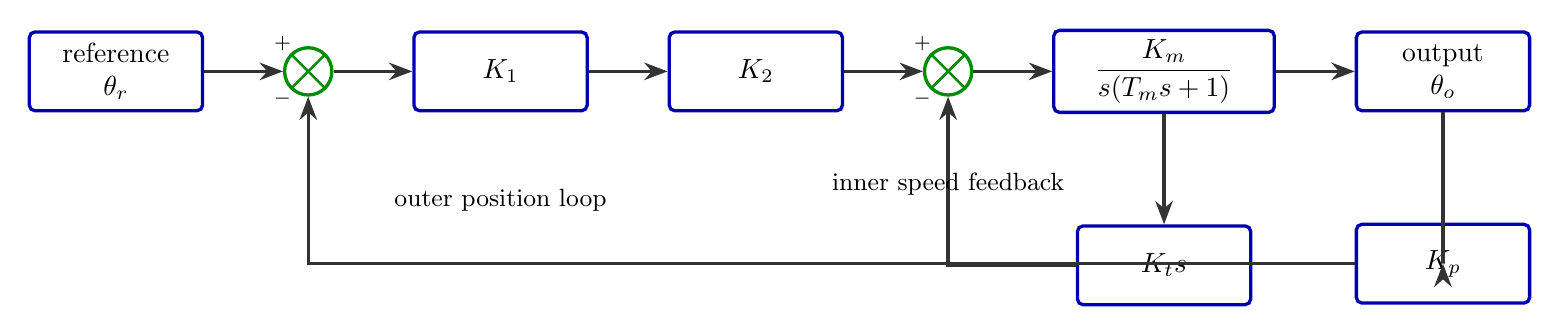
\begin{tikzpicture}[node distance=1.0cm]
  \node[block] (ref) {reference\\$\theta_r$};
  \node[sum, right=of ref] (sum1) {};
  \node[block, right=of sum1] (k1) {$K_1$};
  \node[block, right=of k1] (k2) {$K_2$};
  \node[sum, right=of k2] (sum2) {};
  \node[block, right=of sum2, minimum width=2.8cm] (motor) {$\dfrac{K_m}{s(T_m s+1)}$};
  \node[block, right=of motor] (out) {output\\$\theta_o$};
  \node[block, below=1.4cm of out] (kp) {$K_p$};
  \node[block, below=1.4cm of motor] (kt) {$K_t s$};

  \draw[signal] (ref) -- (sum1);
  \draw[signal] (sum1) -- (k1);
  \draw[signal] (k1) -- (k2);
  \draw[signal] (k2) -- (sum2);
  \draw[signal] (sum2) -- (motor);
  \draw[signal] (motor) -- (out);

  \draw[signal] (out) |- (kp);
  \draw[signal] (kp.west) -| (sum1.south);
  \draw[signal] (motor.south) -- (kt.north);
  \draw[signal] (kt.west) -| (sum2.south);

  \node[font=\scriptsize] at ($(sum1.north west)+(-0.10,0.12)$) {$+$};
  \node[font=\scriptsize] at ($(sum1.south west)+(-0.10,-0.12)$) {$-$};
  \node[font=\scriptsize] at ($(sum2.north west)+(-0.10,0.12)$) {$+$};
  \node[font=\scriptsize] at ($(sum2.south west)+(-0.10,-0.12)$) {$-$};

  \node[note, below=0.85cm of k1] {outer position loop};
  \node[note, below=0.85cm of sum2] {inner speed feedback};
\end{tikzpicture}
\end{document}
